\documentclass[12pt]{article}
\setlength{\textwidth}{17cm}
\setlength{\textheight}{24cm}
\setlength{\topmargin}{-2cm}
\setlength{\footskip}{1cm}
\setlength{\evensidemargin}{0cm}
\setlength{\oddsidemargin}{0cm}
\setlength{\parindent}{0cm}

\usepackage{allrunes}
\usepackage{amsmath}
\usepackage[magyar]{babel}
\usepackage[T1]{fontenc}
\usepackage[utf8]{inputenc}
\usepackage{fixltx2e}
\usepackage{multirow}

\usepackage[hyphens]{url}
\usepackage[unicode,colorlinks=true,breaklinks]{hyperref}
%\usepackage[dvips]{hyperref}
%should display links, but it does not work with \H accent
%and formulas in section titles

\hypersetup{colorlinks,linkcolor=blue,urlcolor=magenta,citecolor=magenta}
%Breaks long url`s in text, while keeping it one link:

\usepackage{amsfonts}
\usepackage{amsthm}
\usepackage{amssymb}


\theoremstyle{plain}
\usepackage{graphicx}

%\usepackage{gensymb}
\usepackage{float}

% For bra-ket notation
\usepackage{braket}

%% New commands
\newcommand{\dd}{\textrm{d}}

%% Pauli matrices
\newcommand{\sigx}{\sigma_x}
\newcommand{\sigy}{\sigma_y}
\newcommand{\sigz}{\sigma_z}

\newcommand{\paulix}{
    \left( \begin{array}{cc}
        0 & 1 \\
        1 & 0
    \end{array}
    \right)
}

\newcommand{\pauliy}{
    \left( \begin{array}{cc}
        0 & -i \\
        i & 0
    \end{array}
    \right)
}

\newcommand{\pauliz}{
    \left( \begin{array}{cc}
        1 & 0 \\
        0 & -1
    \end{array}
    \right)
}


\begin{document}
\title{3. tétel}
\author{Kaszás Bálint}

\maketitle


\newpage
\begin{abstract}
    Véletlen számok generálása, numerikus integrálás, Newton-típusú formulák, Gauss-formulák. Monte-Carlo módszer, Markov-lánc Monte-Carlo, hierarchikus bayes-i hálózatok.
\end{abstract}

\section{Véletlen számok generálása}
A természettudományos problémák megoldása során gyakran szükség van, például véletlenszerű természeti jelenségek szimulálásakor, véletlen számok generálására. 
Nyilvánvaló nehézséget jelent, hogy generálást determinisztikus programmal kell végeznünk. 

Tekintsük az $r_1, r_2, r_3, ...$ számok sorozatát. Ezt véletlenszerűnek ({\em randomnak}) mondjuk, hogyha a számok között nincs korreláció. Determinisztikus módszerekkel nem tudunk korrelációmentes sorozatot előállítani, a véletlenszámok között mindenképpen marad korreláció. Ezért, a számítógéppel generált véletlen számok sorozata igazából csupán {\em pszeudorandom}. Ez azt is jelenti, hogy amennyiben ismerjük $r_m$-t és az őt megelőző számokat a sorozatban, kellő energiabefektetéssel meg tudjuk mondani $r_{m+1}$-et is. 
Kifinomultabb generátorokkat használva a korreláció természetesen csökkenthető. Alternatívaként rendelkezésre állnak olyan adatbázisok is, amelyek {\em valódi véletlen számokat} tartalmaznak, például valami véletlenszerű jelenség mérési adatait. Ezekből azonban nem tudunk elég gyorsan véletlen számokat lehívni.

Tekintsük az egyik legegyszerűbb pszeudorandom számokat generáló algoritmust, a {\em lineáris kongruencia generátort}. Az $r_i$ számokat $0 \leq r_i \leq M-1$ intervallumon generáljuk, egy $a$ és egy $c$ állandók választásával. 

\begin{equation}
    \label{lincong}
    r_i \equiv (r_{i-1}a + c) \text{ mod } M
\end{equation}

A hátránya, hogy amint megismétlődik egy korábbi random szám, az egész sorozat ismétlődni fog. Ebben az egyszerű példában az $r_i$ sorozat $M$ lépés után ismétlődik, ez a generátor {\em ciklushossza}. A lineáris kongruencia hátránya továbbá, hogy több dimenzióban nem korrelálatlanok a generált számok, azaz bizonyos síkok mentén helyezkednek el a többdimenziós térben.

A lineáris kongruencia algoritmus akkor működik 'jól', ha a ciklushossz kellően nagy, és az $a$, $c$ paramétereket is elég nagyra választjuk. A gyakorlatban alkalmazott generátorokban tipikusan $M=2^{32}$ \cite{numrecipes}, vagy $M=2^{64}$ \cite{knuth}. 

Megemlítjük, hogy léteznek a lineáris kongruenciánál kifinomultabb algoritmusok is, amik többek között több dimenziós véletlen számokat is elő tudnak állítani. A legnépszerűbb ezek közül a {\em Mersenne-twister} \cite{random}, amely nevét onnan kapta, hogy a ciklushosszát egy Mersenne-prímnek választják.  
\section{Numerikus integrálás}
A numerikus integrálás alapfeladata \cite{landau}, hogy valamilyen tartományon adott, határozott integrál értékét numerikus módszerekkel kiszámítsuk. Erre azért lehet szükség, mert az integrandusnak gyakran nem ismerjük primitív függvényét. 

Általánosan minden módszer leírható úgy, hogy az integrálási tartományban bizonyos helyeken kiértékeljük az integrandust, majd ezeket megfelelő súlyokkal összeadjuk. 
\subsection{Newton-típusú formulák}
A Newton-típusú formulák, vagy Newton-Cotes formulák az integrálási tartományt egyenlő darabokra osztják fel,
\begin{equation}
    \label{nc}
    \int_a^b f(x) \text{d}x  \approx \sum_{i=0}^n w_i f(x_i),
\end{equation}
ahol $a = x_0 < x_1 < ... < x_i < ... < x_n=b$, egyenletesen elhelyezve, és $w_i$ az $i$. integrálási ponthoz tartozó súly, amelyeket különböző alakban vehetünk fel. 

Minden Newton típusú formula azon alapul, hogy az integrált egy köztes, $[x_i, x_{i+1}]$ intervallumon közelítjük, majd a kis intervallumok járulékát összeadjuk. 

A legegyszerűbb ezek közül a {\em trapéz-szabály}, amely $x_i$ és $x_{i+1}$ között lineárisan interpolál:
\begin{equation}
    \label{trap}
    \int_{x_{i}}^{x_{i+1}} f(x) \text{d}x \approx (x_{i+1} - x_i) \frac{f(x_{i+1} + f(x_i))}{2}.
\end{equation}
Kiszámolható az is \cite{error}, hogy az $[x_i, x_{i+1}]$ intervallumon elkövetett numerikus hiba, amit a trapéz szabályt alkalmazva elkövetünk
$$
\Delta I ^{\text{trap.}} = \frac{1}{12}\Delta x^3 f''(\xi),
$$
valamilyen $\xi \in [x_i, x_{i+1}]$-re. Tehát a módszer hibája a függvény második deriváltjának maximumával becsülhető.


Ezt a kis intervallumokra egymás után alkalmazva és a $\Delta x$ jelölést használva az integrálási pontok távolságára
\begin{equation}
    \int_a^b f(x) \text{d}x  = \Delta x  \frac{f(x_0) + f(x_n)}{2} + \sum_{i = 1} ^{n-1}f(x_i)\Delta x.
\end{equation}

A trapéz szabálynál pontosabb formulákat is használhatunk, ezek az elemi intervallumok feletti interpoláció alakjában különböznek. 
A {\em Simpson-szabály} szerint például másodfokú polinommal interpolálunk, és ezért szükség lesz az intervallum közepén kiértékelt függvényértékre is. Megtartva a $\Delta x = x_{i+1} - x_i$ jelölést:
\begin{equation}
    \int_{x_{i}}^{x_{i+1}} f(x) \text{d}x \approx \frac{\Delta x}{3}\left( f(x_i) + 4f(x_i+\Delta x/2) + f(x_{i+1})\right).
\end{equation}
A Simpson-szabály hibáját is kiszámolhatjuk \cite{error}, erre
$$
\Delta I ^{\text{Simps.}} = \frac{1}{90}\left(\frac{\Delta x}{2}\right)^5 f^{(4)}(\xi) 
$$
adódik, szintén valamilyen $\xi \in [x_i, x_{i+1}]$ értékre. 
\subsection{Gauss-formulák}
A Gauss-formulák ehhez képest nem ragaszkodnak az egyenközű függvény-kiértékeléshez. Ha az $f(x)$ integrandusból kiemelünk egy súly-faktort
\begin{equation}
    \label{nc}
    \int_a^b f(x) \text{d}x  = \int_a^b W(x)g(x) \text{d}x \approx \sum_{i=0} ^n w_i g(x_i).
\end{equation}
Az $n$ darab $x_i$ pontok és a $w_i$ súlyok pedig már nem egyenletesek. Úgy választjuk őket, hogy akkor legyen egzakt a módszer, amikor $g(x)$ egy $2n-1$-ed fokú polinom. Mivel a Gauss-formulák a [$-1, 1$] intervallumra vannak megadva, előtte az integrálunkat is át kell transzformálni erre az intervallumra. 

A Gauss-formulák előnye, hogy ugyanannyi függvénykiértékeléssel sokkal pontosabb eredményre vezetnek a Newton-formuláknál. Az integrálási pontok és a súlyok levezetését mellőzzük, ezek rendelkezésre állnak a legtöbb numerikus könyvtárban. 
\section{Monte-Carlo módszer}
A fent vázolt módszerek egyik hátránya hogy több dimenzióra nem, vagy csak rosszul általánosíthatóak. Erre kínál megoldást a {\em Monte-Carlo} módszer, amellyel sok véletlenszám generálásával tudunk tetszőleges dimenziós integrált kiszámítani. A numerikus integráláson túl a Monte-Carlo típusú módszereket használják optimalizálási feladatokra is. A közös ezekben, hogy {\em véletlen számok segítségével oldanak meg egy determinisztikus problémát}. Tekintsük most a numerikus integrálás esetét. A legegyszerűbb példaként az egységsugarú kör területének kiszámítását tárgyaljuk. Az egyszerűség kedvéért vegyük csak az egyik negyedét a körnek, amit az egységnégyzetbe tudunk beleírni. 

Hogyha az egységnégyzet belsejében {\em egyenletes eloszlással} pontokat generálunk, a negyedkör belsejébe eső pontok számának, és az összes generált pont számának aránya a körcikk területét közelíti. A generált pontok számának növelésével tetszőleges pontosság elérhető. A módszert a \ref{fig:1}. Ábra mutatja. 
\begin{figure}[h!]
    \centering
    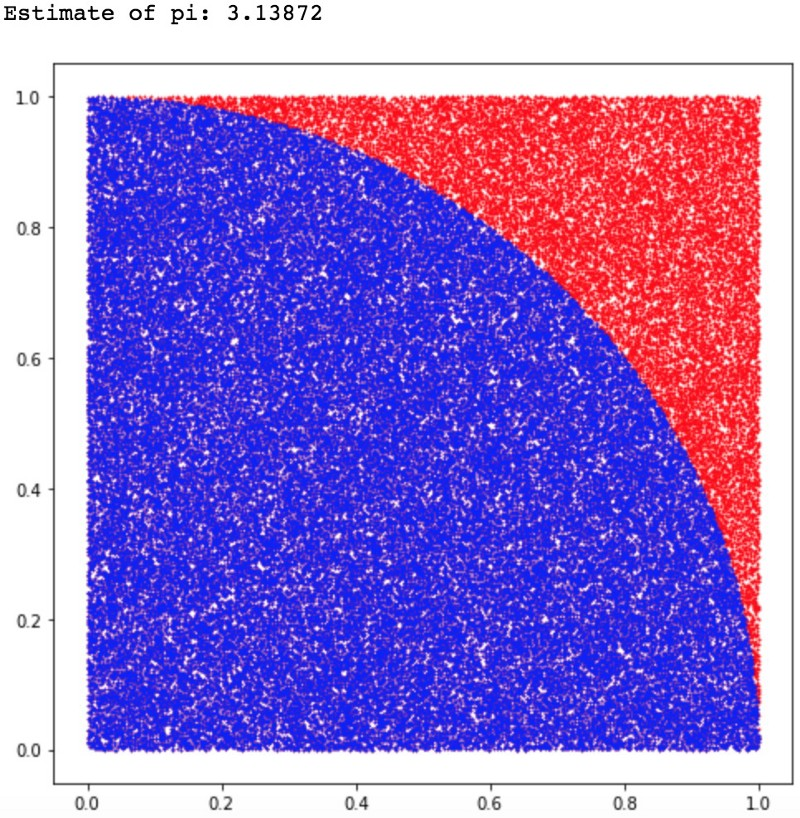
\includegraphics[width = 0.49\textwidth]{media/ht.jpeg}
    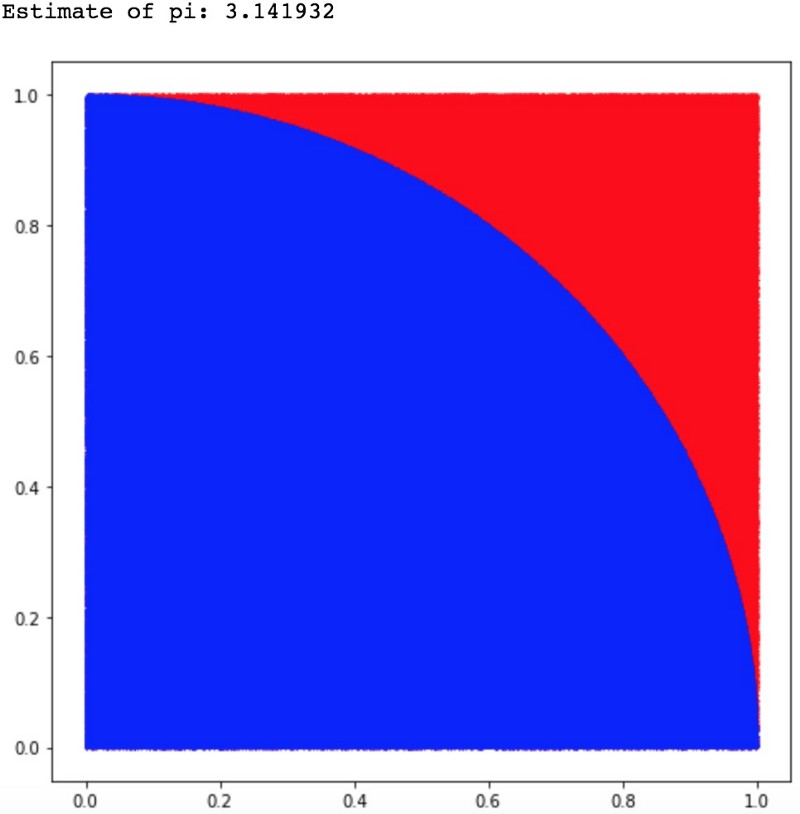
\includegraphics[width = 0.49\textwidth]{media/million.jpeg}
    \caption{A körcikk területének kiszámítása Monte-Carlo módszerrel. Kék pontok jelölik a körcikk belsejébe esett pontokat. A bal panelen $10^5$ pont van elosztva az egységnégyzetben, a jobb panelen pedig $10^6$. Felettük pedig $\pi$ kiszámolt közelítő értéke látható, vagyis a körcikk területének négyszerese. Forrás: \cite{mc}. }
    \label{fig:1}
\end{figure}
Ez a területszámítási (vagy térfogat, magasabb dimenzió esetén) módszer egyszerűen működik tetszőleges alakzatokra is, csupán véletlen pontokról kell eldönteni, hogy bele esnek-e a kívánt tartományba. 

A határozott integrál kiszámítására való alkalmazáshoz a következő szemléletes tulajdonságot használjuk ki. 

\begin{equation}
    I = \int_a ^b f(x) \text{d}x = (b-a)\langle f \rangle
\end{equation}
Vagyis a függvény {\em átlagát} kell kiszámítanunk az intervallumon. Természetesen ez igaz több dimenzióra is, ilyenkor az integrál értéke a tartomány térfogatának és a függvény átlagának szorzata. 

A függvény átlagát pedig már számolhatjuk a Monte-Carlo módszerrel, azaz 
\begin{equation}
    \langle f \rangle  \approx \frac{1}{N}\sum_{i=1}^N f(x_i), 
\end{equation}
ahol $x_i \in [a, b]$ számokat egyenletes eloszlással húzzuk az integrálási tartományból. A minták számának növelésével az $N$ számból számolt átlag a függvény átlagértékéhez tart. A relatív hiba pedig $1/\sqrt{N}$ szerint csökken.  

Az átlagérték kiszámítása lassan változó függvények esetén tényleg egy hatékony módját adja a keresett integrál közelítésének. Azonban mivel egyenletes eloszlású pontokkal dolgozunk, egy gyorsabban változó függvény esetén már nem ad megbízható eredményt, hiszen az egyenletes mintavételezés könnyen kihagyhatja azokat a részeit a függvénynek, ahonnan nagy járulék jönne az átlagba. Erre a problémára, a Monte-Carlo 'megjavítására' két alapvető módszer van:
\subsection{Szórás csökkentés}
Tegyük fel, hogy az integrálandó $f(x)$ függvényhez találunk egy $g(x)$-et, amellyel $f(x)-g(x)$ szórása kicsi, és ismerjük $g(x)$ integrálját.
$$
\int_a ^b g(x) \text{d} x = J.
$$
Így $f(x)-g(x)$ integrálját már számolhatjuk Monte-Carló módszerrel, és a keresett $I$ integrál
$$
I = \int_a ^b f(x) \text{d}x = \int_a ^b f(x)-g(x) \text{d}x + J. 
$$
\subsection{Importance sampling}
A másik megoldás, hogy az egyenletes mintavételezés helyett úgy választjuk a pontokat, hogy azok főleg a függvény nagy járulékot adó részeiről legyenek. Ehhez kifejezzük $I$ integrált egy $w(x)$ súlyfaktorral
\begin{equation}
    I = \int_a ^b f(x) \text{d}x = \int_a ^b w(x)\frac{f(x)}{w(x)}\text{d}x.
\end{equation}
Hogyha pedig $w(x)$-szerint húzunk $x_i$ mintákat, vagyis ezt {\em használjuk valószínűségi eloszlásnak} (az egyenletes helyett), az integrált megkaphatjuk
$$
I = \left \langle \frac{f}{w} \right \rangle \approx \frac{1}{N} \sum_{i=1}^N \frac{f(x_i)}{w(x_i)}. 
$$

\section{Markov-lánc Monte-Carlo módszer}
Az importance sampling kapcsán felmerül az igény arra, hogy tetszőleges eloszlásból generáljunk véletlen számokat. Ez bonyolult feladat is lehet, hogyha a direkt mintavételezés nem opció, vagy nagyon számításigényes (különösen magas dimenziós eloszlások esetén). Erre nyújtanak megoldást a Markov-lánc Monte-Carlo módszerek (MCMC). Nevüket onnan kapták, hogy egy megfelelő határeloszlással rendelkező Markov-Lánc szimulálásával kapjuk a keresett mintát. 
\subsection{Metropolis-Hastings algoritmus}
Egy példa az MCMC algoritmusokra a Metropolis-Hastings algoritmus, amely szerepet kap a termodinamikai szimulációkban is (lásd 4. tétel). 

Az algoritmussal egymás után generálunk véletlen pontokat, méghozzá úgy, hogy minél több pontot generálunk, az eloszlásuk annál jobban közelíti a keresett valószínűségi eloszlást. A pontokat iteratívan kapjuk, a következő pont mindig csak az előzőtől függ (így válik Markov-lánccá). 
Az aktuális pontból kiindulva választunk egy lehetséges új pontot. Ezt a lehetséges új pontot pedig egy megadott valószínűséggel {\em fogadjuk el}, egyébként elutasítjuk. 

Az algoritmus a következő, amennyiben $f(x)$ eloszlással szeretnénk mintákat generálni.
\begin{itemize}
    \item Választunk egy kezdeti $x_0$ pontot és egy $g(x)$ eloszlást, amelyből könnyű mintavételezni. Ezt fogjuk arra használni, hogy új lehetséges mintákat húzzunk. 
    \item Az $n.$ iterációs lépésben:
    \item Válasszunk $g(x)$ szerint egy $x'$ pontot
    \item Számoljuk ki az $\alpha = f(x')/f(x_n)$ hányadost
    \item $x'$-t $\alpha$ valószínűséggel fogadjuk el, azaz húzzunk egy $u$ számot egyenletesen $[0,1]$ között. 
    \item $u\leq \alpha$  esetén elfogadjuk $x'$-t, azaz $x_{n+1} = x'$.
    \item $u > \alpha$ esetén pedig elutasítjuk, $x_{n+1} = x_n$.
\end{itemize}
\section{Hierarchikus bayes-i hálózatok}
A bayes-i hálózat egy olyan statisztikai modell, amelyben a változók egy irányított gráfba rendeződtek, ezzel kifejezve az ok-okozati viszonyt, illusztrációként lásd a \ref{fig:2}. ábrát.  
\begin{figure}[h!]
    \centering
    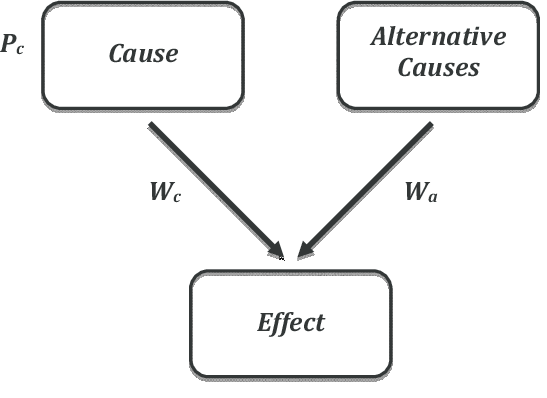
\includegraphics{media/bayes.png}
    \caption{Általános bayes-i hálózat, irányított gráfba rendezve.}
    \label{fig:2}
\end{figure}
Tegyük fel, hogy a mért $x$ adatainkhoz egy paramétert rendelünk, és annak a valószínűségét keressük (posterior), hogy a paraméter értéke $\Theta$, a mért $x$ adatainkat feltéve. Bayes-tétele alapján ez a valószínűség
\begin{equation}
    \label{bayes}
    p(\Theta | x) \sim p(x | \Theta) p(\Theta),
\end{equation}
ahol $p(x|\Theta)$ a likelihood (a megfigyel empirikus eloszlása $x$-nek),  és $p(\Theta)$ $\Theta$ prior eloszlása. 

Egy hierarchikus bayes-i hálózatban azonban $\Theta$ is függhet további paraméterektől (további, őt okozó változóktól), például $\varphi$-től. Ekkor a $\Theta$ prior eloszlását $p(\Theta | \varphi)$ váltja le, vagyis
\begin{equation}
    p(\Theta, \varphi | x) \sim p(x | \Theta) p(\Theta | \varphi ) p(\varphi). 
\end{equation}
A folyamatot addig ismételjük, amíg a felállított statisztikus modell, a bayes-i hálózat minden csúcsát bele nem számoltuk a posterior valószínűségbe. Ezt a posterior eloszlást, vagyis a paraméter eloszlását a gyakorlatban Markov-Lánc Monte-Carlo módszerrel számoljuk ki. A paraméterekre feltett prior eloszlásokból és a likelihood-okból mintákat húzva, előállítjuk a keresett szorzatot. 
\bibliographystyle{plain}
\bibliography{references}

\end{document}
